\documentclass{article}

\usepackage{amsmath}
\usepackage{amssymb}
\usepackage{hyperref}
\usepackage{url}
\usepackage{graphicx}
\usepackage{geometry}
\usepackage{enumitem}
\usepackage{parskip}
\usepackage{chemfig}
\usepackage{pdfpages}
\usepackage{xcolor}
\usepackage{tikz}
\usepackage{fancybox}
\usepackage{makecell}
\usepackage{pgfplots}
\usepackage{soul}
\usepackage{ulem}
\usepackage{wrapfig}
\usepackage{subcaption}
\usepackage[T1]{fontenc}
\usepackage{esvect}
\usepackage{multirow}
\usepackage{booktabs}
\usepackage{float}
\usepackage{tocloft}
\usepackage{caption}
\usepackage{colortbl}
\usepackage{siunitx}
\usetikzlibrary{arrows}
\usetikzlibrary{decorations.pathreplacing}
\pgfplotsset{compat=1.17}
\usepgfplotslibrary{statistics}
\definecolor{darkgray}{rgb}{0.2, 0.2, 0.2}

% === BIBLIOGRAPHY ===
\usepackage[utf8]{inputenc}
\usepackage{csquotes}
\usepackage[style=apa, backend=biber, doi=true, url=true]{biblatex}
\addbibresource{ref.bib}
\DeclareFieldFormat[article]{volume}{\textbf{#1}}
\DeclareFieldFormat[article]{journaltitle}{\textit{#1}}
% ====================
 
\geometry{
    a4paper,
    total={170mm, 257mm},
    left=20mm,
    top=20mm
}

\hypersetup{
    colorlinks=true,
    linkcolor=black,
    urlcolor=blue,
    pdftitle={Report SW10 - EnCheBio}
}

\newcommand{\figbox}[1]{ 
    \begin{figure*}[ht!]        
        \begin{center}            
            \fbox{#1}        
        \end{center}    
    \end{figure*}
}

\newcommand{\wrapfill}{
    \par
    \ifnum \value{WF@wrappedlines} > 0
        \addtocounter{WF@wrappedlines}{-1}%
        \null\vspace{
            \arabic{WF@wrappedlines}
            \baselineskip
        }
        \WFclear
    \fi
    \phantom{}
}

\newcommand{\cfig}[1]{%
  \begin{figure*}[ht!]%
    \centering%
    #1%
  \end{figure*}%
}

% === LIST OF EQUATIONS ===
\newcounter{myequation}
\renewcommand{\themyequation}{\arabic{myequation}}

\newlistof{myequations}{loe}{\Large List of Equations}
\newcommand{\addequationtotoc}[1]{\addcontentsline{loe}{myequations}{\protect\numberline{\themyequation}#1}}

\renewcommand{\cftmyequationspresnum}{}
\renewcommand{\cftmyequationsaftersnum}{\hspace{1em}}
\setlength{\cftmyequationsnumwidth}{2em}
\cftsetindents{myequations}{1.5em}{2.3em}

\newcommand{\capeq}[3]{
    \refstepcounter{myequation}
    \begin{equation*}
        #1
    \end{equation*}
    \label{#2}
    \begin{center}
        \vspace*{-.4cm}
        \noindent{Equation \themyequation:} #3
    \end{center}
    \addequationtotoc{#3}
}

\newcommand{\refeq}[1]{\hyperref[#1]{[Equation~\ref*{#1}]}}
% =========================

\newcommand{\difference}{\,\backslash\,}
\newcommand{\rem}{\underline{Remark}: }
\newcommand{\nots}{\underline{Notation}: }
\newcommand{\prf}{\underline{Proof}: }
\newcommand{\exs}{\underline{Example}: }
\newcommand{\defs}{\underline{Definition}: }
\newcommand{\wrn}{\underline{Warning}: }
\newcommand{\sht}{\ |\ }
\newcommand{\pph}[1]{\paragraph{#1}\phantom{}\\}

% === TEXT ===
\begin{document}

\hypersetup{citecolor=black}

\begin{minipage}{0.7\textwidth}
    \vspace*{-.8cm} \hspace*{-0.3cm}
    
\includegraphics[width=.5\textwidth]{media/hslu-logo.png}
\end{minipage}

\vspace*{2cm}

\textbf{\huge Practical 3:}\\[.75cm]
\begin{center}
    \textbf{\huge Analysis of PAHs in Plastics}
    
    \textbf{\huge by GC-MS}\\[1cm]
    
    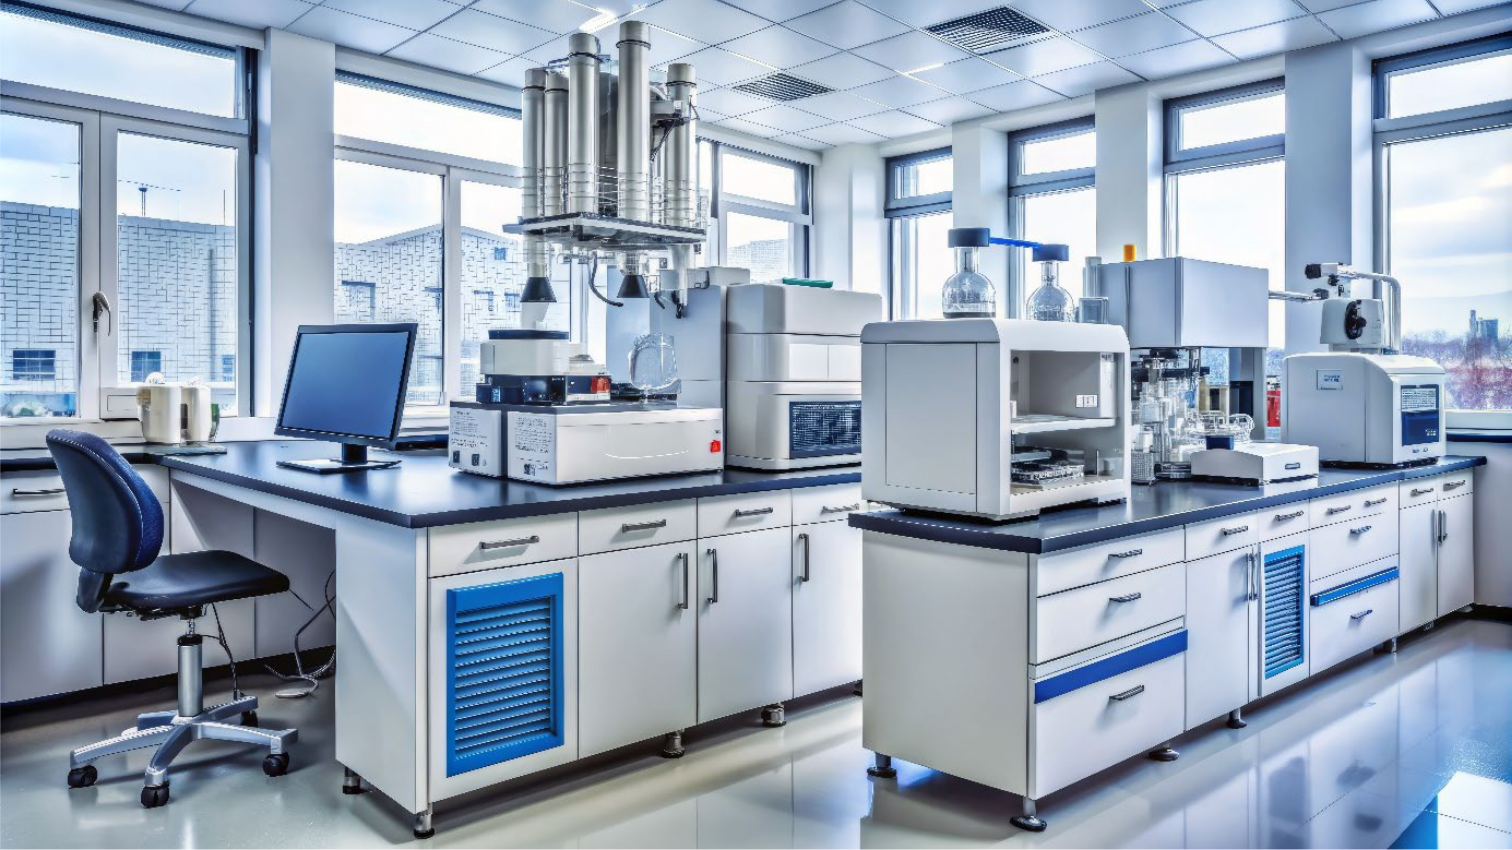
\includegraphics[width=\textwidth]{media/front_practical3.png}\\
\end{center}

\vfill

\setlength{\intextsep}{0pt}%
\begin{wrapfigure}{r}{\textwidth}
    \textbf{\Large Environmental Chemistry and Biology HS2024\\[.5cm]
    \large Dr. Macarena San Martín Ruiz\\
    Lecturer}
    \vspace{-2.1cm}
\end{wrapfigure}

\phantom{}\\[-1cm]

\begin{flushright}
        \large
        \textbf{Team 4}\\
        Matteo Frongillo\\
        Ramadhan Nura\\
        Folagbade Popoola\\
        Jonathan Lawrence Boms\\
        Kron Xhemajli
\end{flushright}
\wrapfill
\newpage
\tableofcontents
\pagebreak

\section{Introduction}
The purpose of this experiment is to understand the analysis and quantification of polycyclic aromatic hydrocarbons (PAHs) in plastics using Gas Chromatography-Mass Spectrometry (GC-MS). This involves learning key concepts such as chromatographic separation, detection techniques, and calibration methods.

\section{Materials and Methods}
\subsection{Materials}
\begin{itemize}
    \item Gas chromatograph (Agilent Technologies GC 6890N)
    \item Mass spectrometer (Agilent MSD 5973)
    \item Supelco SLB-5 ms column (30 m $\times$ 250 $\mu$m $\times$ 0.25 $\mu$m)
    \item Helium (carrier gas)
    \item Standard PAH kit
    \item Acetonitrile (solvent)
    \item Pipettes and vials
\end{itemize}

\subsection{Experimental Procedure}
\begin{enumerate}
    \item \textbf{Sample Preparation:} Prepare dilutions from a 10 $\mu$g/mL stock solution using the formula \(C_1V_1 = C_2V_2\) to achieve concentrations of 1 $\mu$g/mL, 0.1 $\mu$g/mL, and 0.01 $\mu$g/mL.
    \item \textbf{GC-MS Setup:} Set the column temperature program to start at \SI{70}{\degreeCelsius}, increase at \SI{5}{\degreeCelsius}/min to \SI{350}{\degreeCelsius}, and hold for 5 minutes.
    \item \textbf{Injection:} Inject 1 $\mu$L of each dilution into the GC-MS system in split mode.
    \item \textbf{Data Acquisition:} Record chromatograms, noting retention times, peak areas, and mass spectra for each PAH.
    \item \textbf{Calibration Curve:} Use the standard solutions to construct a calibration curve by plotting peak area against concentration.
\end{enumerate}

\section{Results}
\subsection{Calibration Data}
\begin{table}[H]
    \centering
    \caption{Calibration data for Chrysene}
    \begin{tabular}{@{}cccc@{}}
        \toprule
        \textbf{Concentration (ng/mL)} & \textbf{Peak Area} & \textbf{Retention Time (min)} & \textbf{m/z Fragments}\\
        \midrule
        1000 & 1025 & 8.5 & 228\\
        100  & 520 & 8.5 & 228\\
        50   & 260 & 8.5 & 228\\
        10   & 105 & 8.5 & 228\\
        5    & 50  & 8.5 & 228\\
        \bottomrule
    \end{tabular}
    \label{tab:calibration-data}
\end{table}

\subsection{Chromatograms}
Include chromatograms here with appropriate annotations.

\subsection{Unknown Sample Analysis}
The peak area for the unknown sample was 300. Using the calibration curve equation, the concentration is determined as:
\capeq{C = \frac{(300 - 0)}{12} = 25\, \text{ng/mL}}{eq:concentration}{Concentration of Chrysene in the unknown sample}

\section{Discussion}
\begin{itemize}
    \item Discuss the separation efficiency, retention times, and peak identification.
    \item Answer questions on compound appearance order, fragmentation, and hydrophobicity.
    \item Explain the differences between the calibration curve method and the internal standard method.
\end{itemize}

\section{Conclusion}
This experiment provided a hands-on understanding of GC-MS analysis for PAHs, highlighting the importance of calibration and method validation for accurate quantification.

\printbibliography

\end{document}